\documentclass[11pt]{article}
\usepackage[a4paper,margin=1in]{geometry}
\usepackage{hyperref}
\usepackage{enumitem}
\usepackage{parskip}
\usepackage{graphicx}
\usepackage{booktabs}
\usepackage{tabularx}

\hypersetup{colorlinks=true,urlcolor=blue,linkcolor=black}
\setlist{nosep,leftmargin=*}

\title{\vspace{-2em}CS5013 Mid-demo Report\\[0.3em]
\large Exchange Student Guide \& Community Platform}
\author{Mikhail Novikov, Roll no.\ GE26Z858 \and Abdirakhim Ismailov, Roll no.\ GE26Z860}
\date{9 October 2026}

\begin{document}
\sloppy
\maketitle

\vspace{-1em}
\noindent\rule{\textwidth}{0.4pt}

\noindent Repository: \url{https://github.com/rikire/Exchange-Student-Guide-Platform}. As in the
design document, every figure below names the file or command it comes from, so it can be checked
against the repository rather than taken on trust.

\vspace{0.4em}
\noindent\begin{tabularx}{\textwidth}{@{}llX@{}}
\toprule
\textbf{What the rubric asks} & \textbf{Section} & \textbf{Evidence in the repository} \\
\midrule
Core workflow on a real input & \S1 & \texttt{docs/course/mid-demo.md} \\
Both members contributing across weeks & \S2 & \texttt{scripts/contribution.sh}, \texttt{docs/team/} \\
An honest gap list & \S3 & \texttt{docs/gap-list.md}, \texttt{docs/tech-debt.md} \\
Explaining any part of the code & \S4 & \texttt{docs/ai/journal/}, \texttt{docs/verification/} \\
\bottomrule
\end{tabularx}

\noindent\rule{\textwidth}{0.4pt}

\section{The core workflow runs end to end on a real input}

The scenario of the proposal: a student searches for ``FRRO registration'', reads the article,
follows a wiki link, proposes an edit with a photo of a paper form; the OGE moderator approves it,
and the change is live. The real input is the guide's seed: 38 articles written from OGE's
International Student Handbook 2026, each citing its pages (\texttt{app/src/main/resources/data/seed/}).
\emph{Registering with FRRO} is one of them.

\noindent\begin{tabularx}{\textwidth}{@{}rlXl@{}}
\toprule
\# & \textbf{Who} & \textbf{Step and what is seen} & \textbf{Requirement, test} \\
\midrule
1 & Student & The landing page: search box, pinned articles & FR-009, \texttt{LandingControllerTest} \\
2 & Student & ``FRRO registration'' returns \emph{Registering with FRRO} first & FR-007, \texttt{SearchFlowTest} \\
3 & Student & The article, rendered from Markdown, with its tags & FR-001, \texttt{ArticleControllerTest} \\
4 & Student & The wiki link \emph{your student visa} opens \emph{Applying for Your Student Visa} & FR-002, \texttt{WikiLinkRendererTest} \\
5 & Student & \emph{Propose an edit}: a sentence and a photo; a submission number; the article unchanged & FR-011, \texttt{SubmissionFlowTest} \\
6 & Moderator & Signs in; the edit at the top of the queue & FR-014, \texttt{ModerationFlowTest} \\
7 & Moderator & The change as a diff of the text as read, and the photo & FR-015, FR-029 \\
8 & Moderator & \emph{Approve \& publish}: the sentence and the photo are live, and found by search & FR-017, FR-032 \\
\bottomrule
\end{tabularx}

Run on 9 October on a stand reset from scratch (\texttt{docker compose down -v}, then
\texttt{up --build}: 38 articles imported, the search index built at start), in Chrome; the edit
was \texttt{SUB-T55S-85MK-2E85}, the photo a drawing of Form C.

\begin{figure}[h]
\centering
\begin{tabular}{@{}cc@{}}
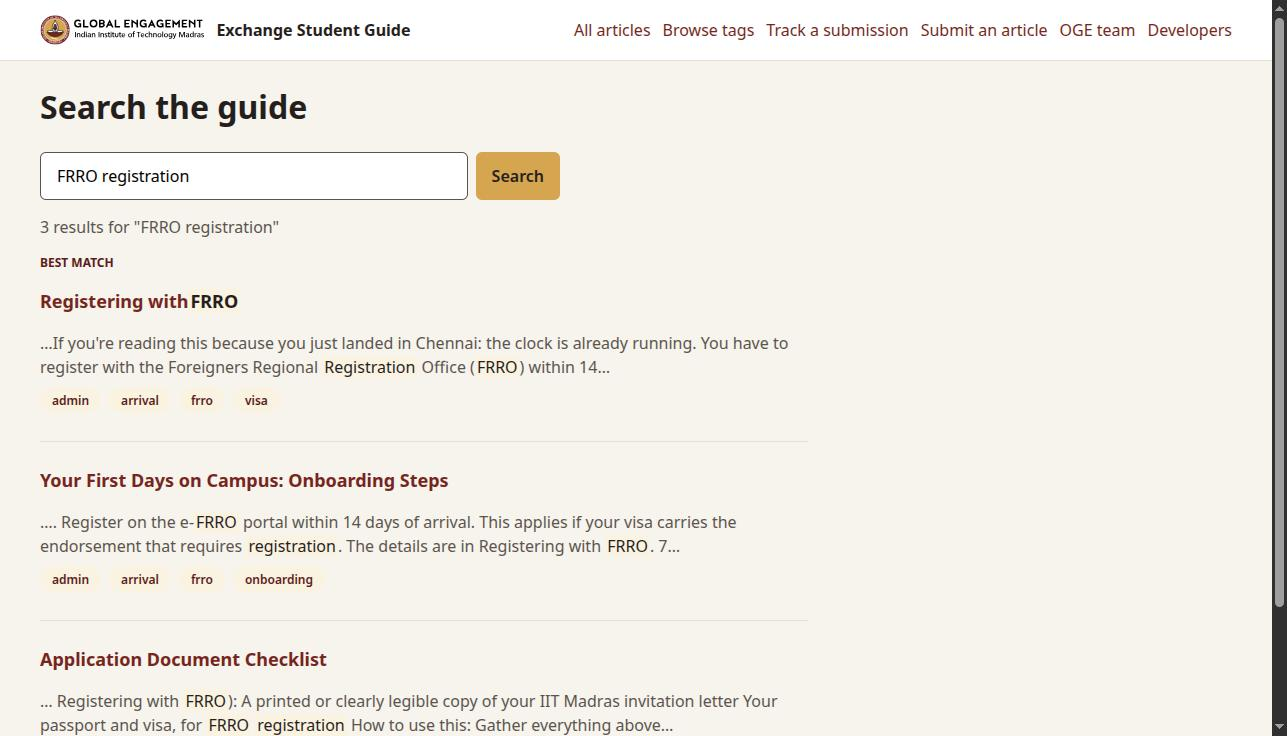
\includegraphics[width=0.48\textwidth]{mid-demo-report/2-search.jpg} &
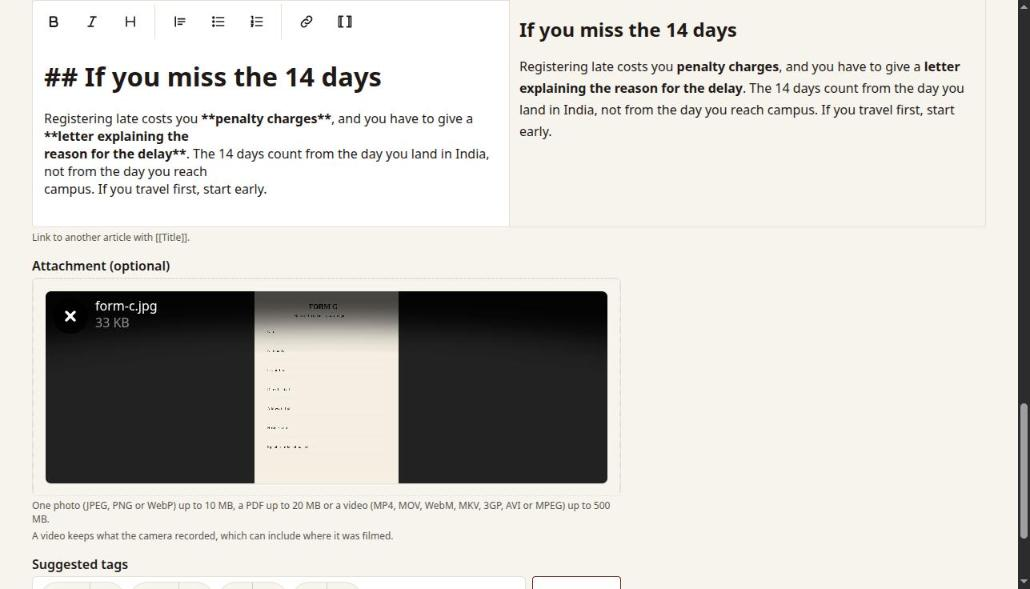
\includegraphics[width=0.48\textwidth]{mid-demo-report/5-edit-form.jpg} \\
\small 2. ``FRRO registration'', the article first & \small 5. The edit: the photo previewed \\[0.6em]
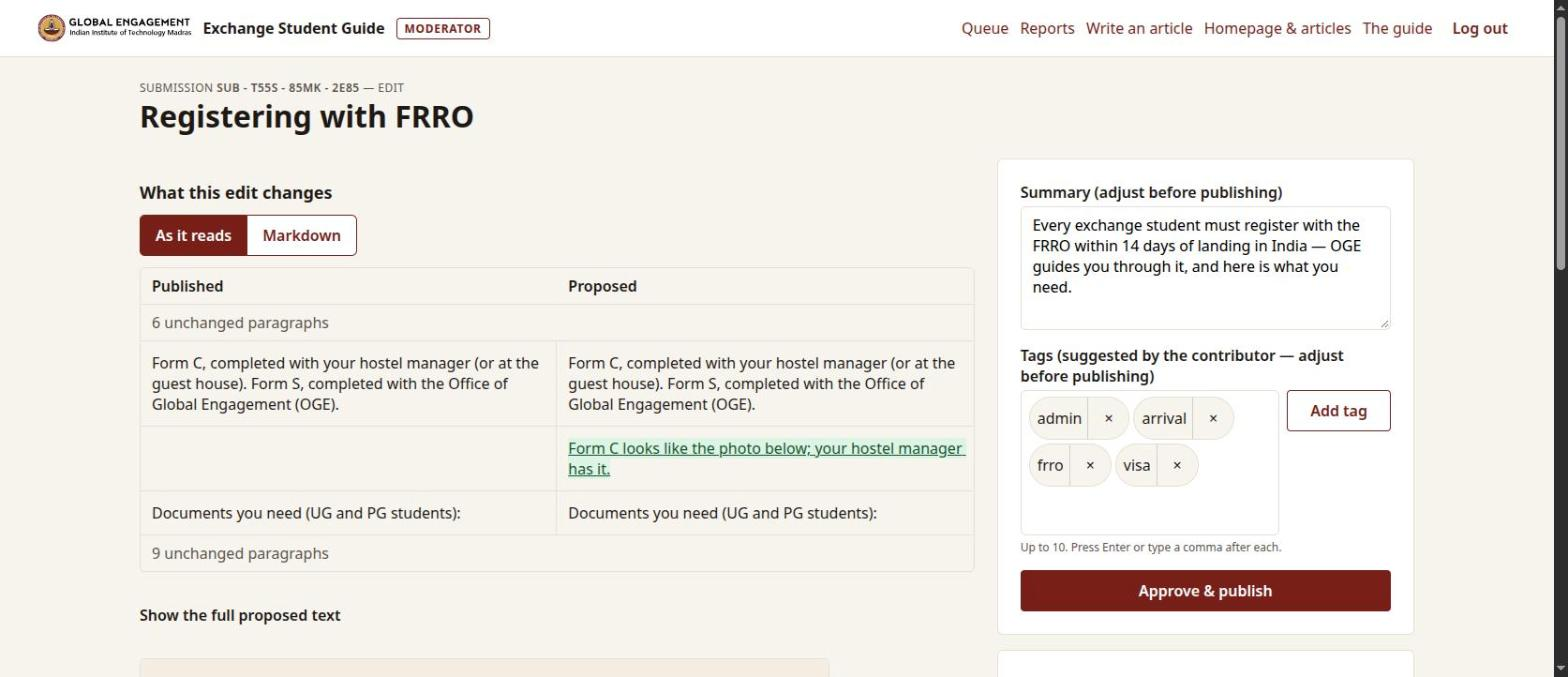
\includegraphics[width=0.48\textwidth]{mid-demo-report/7-review.jpg} &
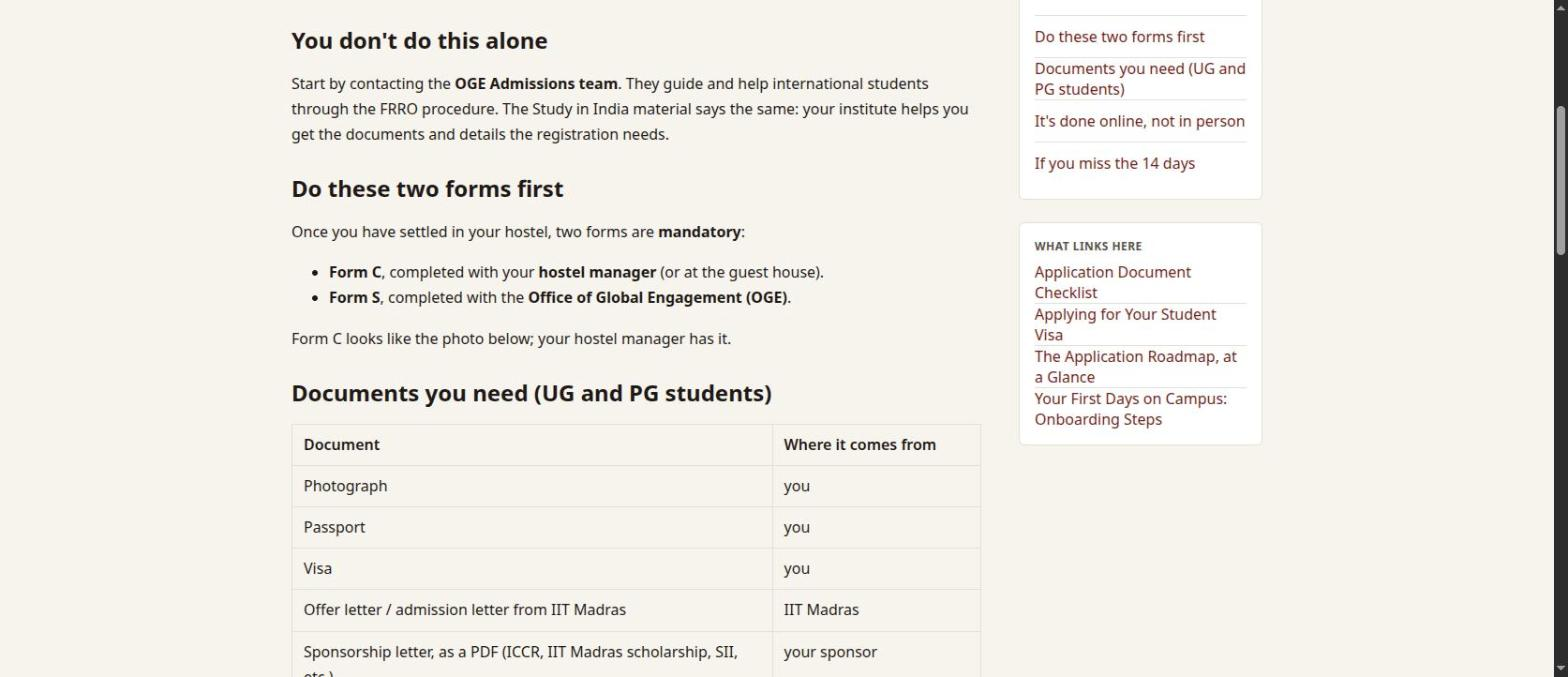
\includegraphics[width=0.48\textwidth]{mid-demo-report/8-published.jpg} \\
\small 7. The moderator's diff of the text as read & \small 8. The sentence live in the article \\
\end{tabular}
\end{figure}

\subsection*{The rehearsal found what the tests could not}

On 4--5 October the scenario was run on the Docker Compose stand, with PostgreSQL and the volumes an
earlier version had filled, rather than on the in-memory database the tests use
(\texttt{docs/roadmap/03-main-flow.md}). Four faults surfaced that none of the 635 application
tests could see: two lived in what an older image had left on disk, one in a page no test asked
for, and one in a mouse click:

\begin{itemize}
\item The stand did not start: since the image runs as an unprivileged user, the volumes written
  by the earlier root image were read-only to it. Recorded as \texttt{DEBT-026}, with the one-off
  fix.
\item The approval answered \texttt{500}: the search index on disk predated a change to its fields,
  and was kept because it held documents. Since 5 October it is rebuilt at every start, a reversal
  recorded as an amendment to ADR-0004.
\item That \texttt{500} was Tomcat's bare page: no generic error page existed. Added, with a test.
\item After a tag was added with Enter, its list of suggestions stayed open over \emph{Submit for
  review}, so a click there added a tag and sent nothing. Fixed, with the browser test that would
  have caught it.
\end{itemize}

After the fixes the scenario ran end to end on the stand. The demo itself is given later; the
stand is reset before it (\texttt{docker compose down -v}).

\section{Both members contribute, across weeks}

Authored commits per ISO week, from \texttt{sh scripts/contribution.sh}. Journal entries written by
the \texttt{Stop} hook are counted apart and never added in.

\noindent\begin{tabular}{@{}lrrrrrrr@{}}
\toprule
& W35 & W36 & W37 & W38 & W39 & W40 & W41 (to 9 Oct) \\
\midrule
Mikhail & 1 & 36 & 34 & -- & 63 & 34 & 11 \\
Abdirakhim & -- & 8 & 9 & -- & 39 & 174 & 25 \\
\bottomrule
\end{tabular}

Two things this table shows that we do not hide. Week 38 (14--20 September) has no commits from
either of us; the weekly log for it is still to be agreed (\texttt{docs/team/weekly-log/}). And the
split is uneven by area: \texttt{docs/team/ownership.md}, generated from the same history, gives
Abdirakhim more commits in twelve of the thirteen application slices, while Mikhail built the
process layer (\texttt{tools/}, 132 commits: the prompt journal, the guards, the generators of the
gap list, traceability and ownership) and, in the application, the contributor's forms of fix 3.6.

\section{The gap list is honest because nobody writes it}

\texttt{docs/gap-list.md} is generated by \texttt{java -jar tools/target/ai-tools.jar gaps} from the
requirements' status, the debt register and the traceability chain, and the pre-push hook refuses a
push while it is out of date. It cannot be trimmed before a demo without changing what it is
generated from.

\begin{itemize}
\item \textbf{Requirements:} 42 of 43 functional and non-functional requirements done; FR-028
  (completing a wiki link while writing, \emph{should}) is planned and has no test.
\item \textbf{Open technical debt:} eight entries, each with its cause, consequence, fix and the
  event that makes it urgent (\texttt{docs/tech-debt.md}).
\item \textbf{Gaps in the chain} from requirement to code to test: none.
\end{itemize}

Two of the open entries are ones neither of us would have volunteered: \texttt{DEBT-026} was found
only by running the stand on old volumes, and \texttt{DEBT-023} records a browser test that failed
twice in full runs of the browser suite and never alone; the likely cause is fixed but not proven,
so the entry stays open.

\section{We can explain any part of the code}

\textbf{How the code was written.} Every prompt, the outcome and the human's own edits are in
\texttt{docs/ai/journal/}, committed by a hook. Before any change the assistant states a contract
(goal, boundaries, criteria, steps) and waits for confirmation; requirements, ADRs, the route
contract and the schema change only with the human's approval. A failing test comes before the
code, and a decision against a library is written down with the reason.

\textbf{What checks it.}
\begin{itemize}
\item 635 application tests and 352 for the tools, on every push (\texttt{scripts/check.sh}); the
  same suite on PostgreSQL 17 in a CI job of its own.
\item 51 browser tests in Chromium through Playwright, with axe for accessibility, at four widths
  from 320 to 1920 pixels.
\item Mutation testing (PIT, by hand before a stage): 132 mutants of the pure logic, 130 killed; the
  two survivors are equivalent and explained (\texttt{docs/verification/mutation-testing.md}).
\item Property-based tests (jqwik) of the address rules and the wiki-link reading, 1000 generated
  titles each in English, Hindi and Tamil.
\end{itemize}

\textbf{What is not ready.} \texttt{docs/viva/} is still a placeholder; preparing it on every slice,
since we take tasks freely rather than owning fixed areas, is part of phase 5.

\section{Since the design document, and what comes next}

The design document of 11 September planned phase 3 as the main flow. It is built: 22 features, 22
ADRs, every slice of the module map now holds code, and \texttt{ModularityTest} still enforces their
boundaries. Ahead, in phase 4 and 5: the meeting with OGE on the working stand, the handoff package
that lets OGE run it without us, the viva preparation, and the open debt, each at its trigger.

\end{document}
